\section{Spatial statistics}

\begin{frame}{Spatial statistics}

  \begin{itemize}
  \item Concerned with data on (at least) 3 variables:
    \begin{itemize}
    \item 2 measure location in space
    \item others measure some features of that location.
    \end{itemize}
  \item Related to GIS (SAS does, \emph{if} you have licence).
  \item Our aim: data at some locations, estimate what data would be
    at larger set of locations.
  \item Summarize in 3D or contour plot.
  \item Concern: data from nearby points probably \emph{correlated}.
  \end{itemize}

\end{frame}


\begin{frame}{A 3D plot}
  Some data with \texttt{x, y} as location, \texttt{z} as height. Draw
  picture of surface:

  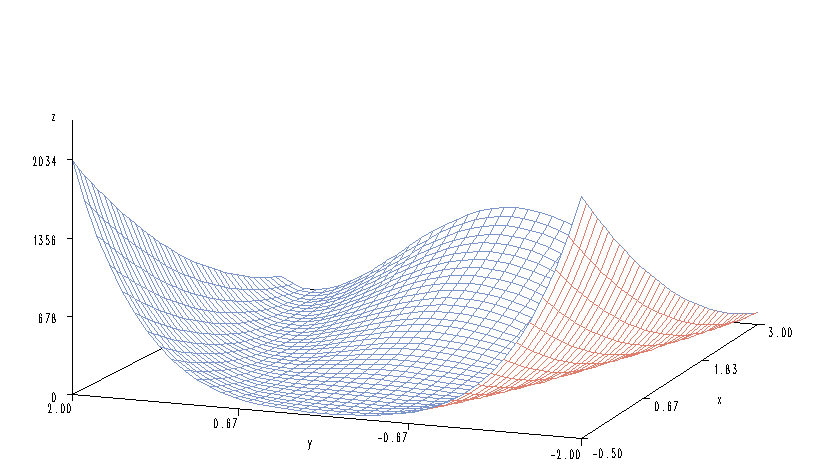
\includegraphics[width=4in]{banana1}


\end{frame}

\begin{frame}{The same, as contour plot}
  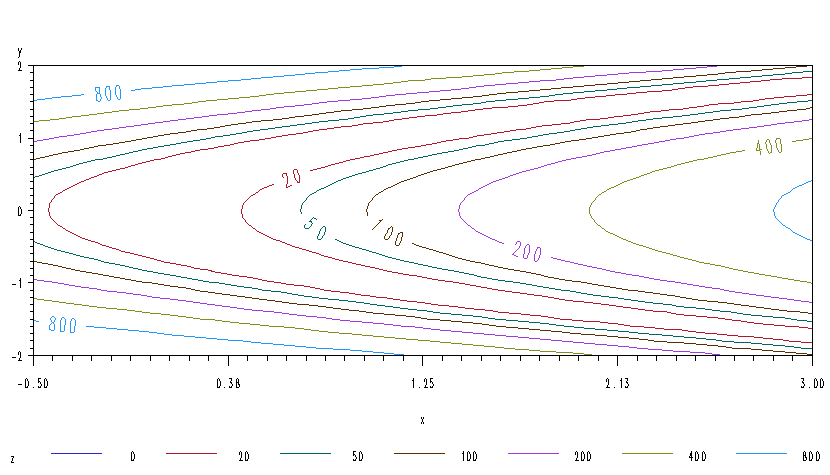
\includegraphics[width=4in]{banana2}
\end{frame}

\begin{frame}{More frequently\ldots}

  \begin{itemize}
  \item have data at set of (possibly irregular set of) locations
  \item want to estimate the surface, and make plot, allowing for
    spatial autocorrelation.
  \item Estimation has two stages:
    \begin{itemize}
    \item estimate autocorrelation structure and nature of any
      anisotropy (\texttt{proc variogram})
    \item feed these into estimation of entire surface (\texttt{proc
        krige2d}), a procedure called \textbf{kriging}.
    \end{itemize}
  \item Kriging based on idea that degree of correlation between pair
    of measurements based only on \emph{distance} between them, not
    direction or absolute locations.
  \end{itemize}
  
\end{frame}


\begin{frame}[fragile]{Example data}

  \begin{itemize}
  \item Thickness of coal seam measured at various locations in a coalfield.
  \item Aim: find where coal seam thickest, most profitable to mine.
  \item Do this by estimating thickness everywhere and making plot.
  \item First step: read in data and make 3D plot:

\begin{verbatim}
data thick; 
  input east north thick @@; 
  datalines; 
   0.7  59.6  34.1   2.1  82.7  42.2   4.7  75.1  39.5  
  ...
  91.5  55.4  39.0  92.9  46.8  39.1  93.4  70.9  39.7  
  94.8  71.5  39.7  96.2  84.3  40.3  98.2  58.2  39.5 
;

proc g3d;
    scatter north*east=thick;

\end{verbatim}
  \end{itemize}
  
\end{frame}

\begin{frame}[fragile]{3D plot of data}

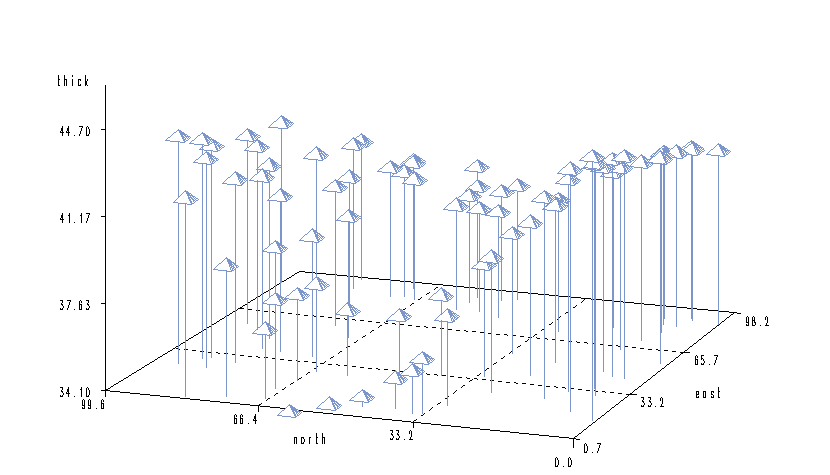
\includegraphics[width=4in]{thick1}

or get (crude) contour plot:

\begin{verbatim}
proc plot;
    plot north*east=thick / contour=5;

\end{verbatim}
  
\end{frame}

\begin{frame}[fragile]{Contour plot}

{\scriptsize
\begin{verbatim}
                          Contour plot of north*east.

north |
  100 +                                                               W
      |                 #   ##              W  W
      |  W                 W        W   W                W            W    W
      |    X             X         W              W     W           X    XX
      |     +    X    X    X      X          X                      XX
      | .                 +                                     X    X  X    X
   50 +    . .              +                                    X     X X
      |       +                X                               X
      |     +    X               X           X            X
      |                  X         W       W       W
      |                  W                          W          W
      |             #        ## #     ## #                W    W   W  WW
    0 +          #                             #                      W
      --+-------------+-------------+-------------+-------------+-------------+-
        0            20            40            60            80            100
                                         east
      Symbol        thick     Symbol        thick     Symbol        thick
      .....   32.5 - 35.0     XXXXX   37.5 - 40.0     #####   42.5 - 45.0
      +++++   35.0 - 37.5     WWWWW   40.0 - 42.5
NOTE: 4 obs hidden.
\end{verbatim}
}

\end{frame}

\begin{frame}{Discussion}

  \begin{itemize}
  \item Could be kind of parabolic surface.
  \item Or: mean height actually \emph{constant} with local deviations
    from it, consistently in same direction as nearby ones (spatial
    autocorrelation).
  \item Hard to tell difference (like time series: is mean changing,
    or is pattern caused by autoregressive/moving average process?)
  \item If there is eg.\ linear trend, fit it first, and work with
    residuals from this regression.
  \end{itemize}
  
\end{frame}

\begin{frame}[fragile]{The variogram, first run}

  \begin{itemize}
  \item Determines whether/how correlation depends on distance.
  \item Needs two options \texttt{lagdistance} and \texttt{maxlags},
    but start with no idea about them. Make SAS run with defaults to
    get sense of what they should be:

\begin{verbatim}
proc variogram;
    compute novariogram;
    coordinates xc=east yc=north;
    var thick;
\end{verbatim}


  
  \end{itemize}
  
\end{frame}

\begin{frame}[fragile]{First run output}

{\scriptsize
\begin{verbatim}
                     Pairwise Distance Intervals

                                           Number
        Lag                                    of    Percentage
      Class    ---------Bounds---------     Pairs      of Pairs

          0          0.00          6.97        45        1.62%
          1          6.97         20.91       263        9.48%
          2         20.91         34.84       383       13.80%
          3         34.84         48.78       436       15.71%
          4         48.78         62.72       495       17.84%
          5         62.72         76.66       525       18.92%
          6         76.66         90.60       412       14.85%
          7         90.60        104.53       179        6.45%
          8        104.53        118.47        35        1.26%
          9        118.47        132.41         2        0.07%
         10        132.41        146.35         0        0.00%

\end{verbatim}
}

\begin{itemize}
\item Max distance between pair of points between 118 and 132. SAS
  divides distances (by default) into $10+1$ classes, and counts \# point
  pairs in each.
\end{itemize}
\end{frame}

\begin{frame}[fragile]{More classes?}
\begin{itemize}
\item Want:
  \begin{itemize}
  \item as many lag classes as possible
  \item at least 30 pairs in each class (except class 0), up to
    reasonable distance.
  \end{itemize}
\item Can certainly use more classes here. Try 30:

\begin{verbatim}

proc variogram;
    compute nhclasses=30 novariogram;
    coordinates xc=east yc=north;
    var thick;
\end{verbatim}

\end{itemize}
  
\end{frame}

\begin{frame}[fragile]{30 classes}

{\tiny
\begin{verbatim}
                    Pairwise Distance Intervals

                                           Number
        Lag                                    of    Percentage
      Class    ---------Bounds---------     Pairs      of Pairs

          0          0.00          2.32         4        0.14%
          1          2.32          6.97        41        1.48%
          2          6.97         11.61        69        2.49%
          3         11.61         16.26        86        3.10%
          4         16.26         20.91       108        3.89%
          5         20.91         25.55       120        4.32%
         ...
         13         58.07         62.72       209        7.53%
         ...
         21         95.24         99.89        60        2.16%
         22         99.89        104.53        30        1.08%
         23        104.53        109.18        19        0.68%
         24        109.18        113.83        11        0.40%
         25        113.83        118.47         5        0.18%
         26        118.47        123.12         1        0.04%
         27        123.12        127.76         1        0.04%
         28        127.76        132.41         0        0.00%
         29        132.41        137.06         0        0.00%
         30        137.06        141.70         0        0.00%
\end{verbatim}
}

\begin{itemize}
\item All right. Usually lag class 1 is limiting factor;
  wouldn't want much smaller.
\end{itemize}
  
\end{frame}

\begin{frame}[fragile]{The next stage}

  \begin{itemize}
  \item Output also includes:

{\scriptsize
\begin{verbatim}
                          Pairs Information

            Number of Lags                              31
            Lag Distance                              4.65
\end{verbatim}
}

\item This is what we want for \texttt{lagdistance}: round up to 5 to
  be safe.
\item \texttt{maxlags} is (a bit less than) highest numbered lag class
  with $\ge 30$ point pairs in it: here 22, round down to 20.
\item Save output data set with variogram in it, print:

\begin{verbatim}
proc variogram data=thick outv = outv; 
  compute lagdistance = 5 maxlag = 20; 
  coordinates xc=east yc=north; 
  var thick;

proc print;

\end{verbatim}

  \end{itemize}
  
\end{frame}

\begin{frame}[fragile]{Output data set}

SAS produces some output, repeated in output data set:

{\tiny
\begin{verbatim}
  Obs VARNAME LAG COUNT DISTANCE AVERAGE  VARIOG  STDERR   COVAR

     1  thick   -1   75     .     40.1387  .       .       5.59592
     2  thick    0    4    1.8919 40.1250 0.04250 0.03005  6.73456
     3  thick    1   51    5.9367 40.4382 0.12363 0.02448  5.54671
     4  thick    2   76   10.1651 40.0428 0.70243 0.11395  3.72434
     5  thick    3  104   15.1243 40.1115 1.31000 0.18166  3.29897
     6  thick    4  123   20.1472 40.0516 2.73240 0.34842  2.68629
     7  thick    5  136   25.3109 39.8081 4.02140 0.48767  1.88510
     8  thick    6  130   29.8661 39.8746 5.16485 0.64062  0.64092
     9  thick    7  150   35.0573 39.8130 5.88077 0.67905 -0.51211
    10  thick    8  137   40.1762 39.9540 7.65146 0.92448 -1.93853
    11  thick    9  163   45.0273 39.8837 6.95408 0.77030 -1.85804
    12  thick   10  165   49.6994 39.8558 7.40564 0.81533 -2.31356
    13  thick   11  159   54.8782 39.8881 7.32824 0.82189 -2.23589
    14  thick   12  219   60.0973 40.0637 7.13244 0.68160 -2.08081
    15  thick   13  194   65.1025 40.2987 6.31673 0.64137 -1.71279
    16  thick   14  180   69.9306 40.2514 5.81919 0.61340 -0.91277
    17  thick   15  190   74.9328 40.3763 5.43221 0.55733  0.05297
    18  thick   16  155   80.1055 40.4206 5.35065 0.60779  0.36238
    19  thick   17  151   85.0293 40.4940 5.15768 0.59358  1.69427
    20  thick   18  117   89.9044 40.2175 6.08030 0.79496  0.98993
    21  thick   19   73   94.6578 40.1733 7.66295 1.26838  0.18459
    22  thick   20   47   99.5352 40.8447 6.61277 1.36411  0.30689

\end{verbatim}
}

\end{frame}

\begin{frame}[fragile]{Discussion}

\begin{itemize}
\item Variogram itself in \texttt{variog}.
\item \texttt{stderr} says how accurately variogram estimated. If too
  big at end, reduce \texttt{maxlag}.
\item Plot should go up to a limit, except for sampling error.
\item Plot:
\begin{verbatim}
proc gplot;
    plot variog*distance;
\end{verbatim}
\end{itemize}
  
\end{frame}

\begin{frame}{Variogram plot}

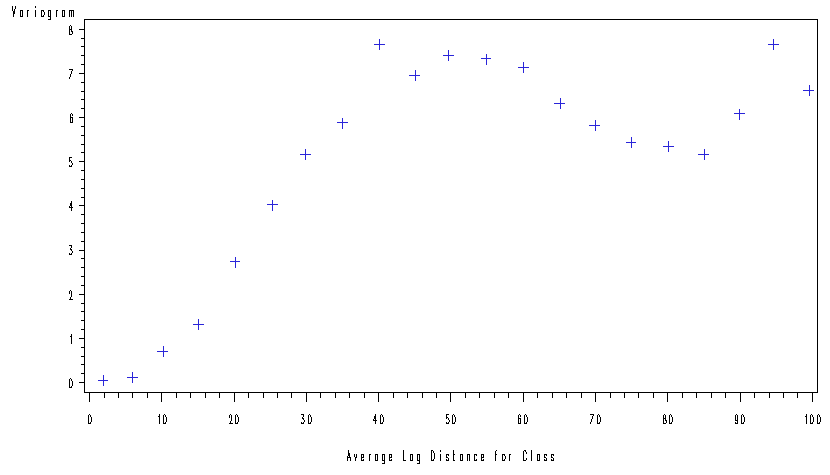
\includegraphics[width=4in]{variog1}

\pause

\begin{itemize}
\item Now need to decide on \textit{shape}.
\end{itemize}
  
\end{frame}

\begin{frame}{Spherical}

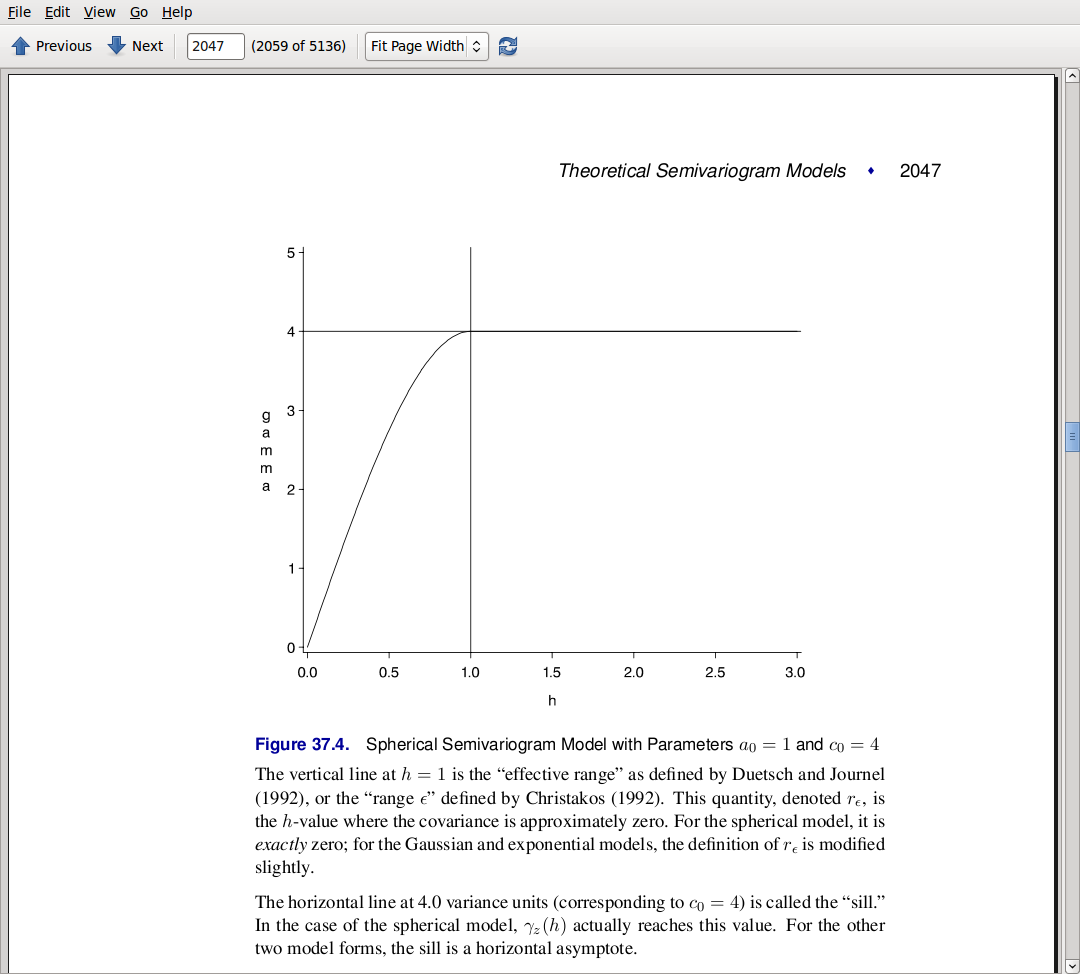
\includegraphics[width=3in]{spherical-model}

Range is 1, scale is 4.

Rises fast, then levels off abruptly.

\end{frame}

\begin{frame}{Exponential}

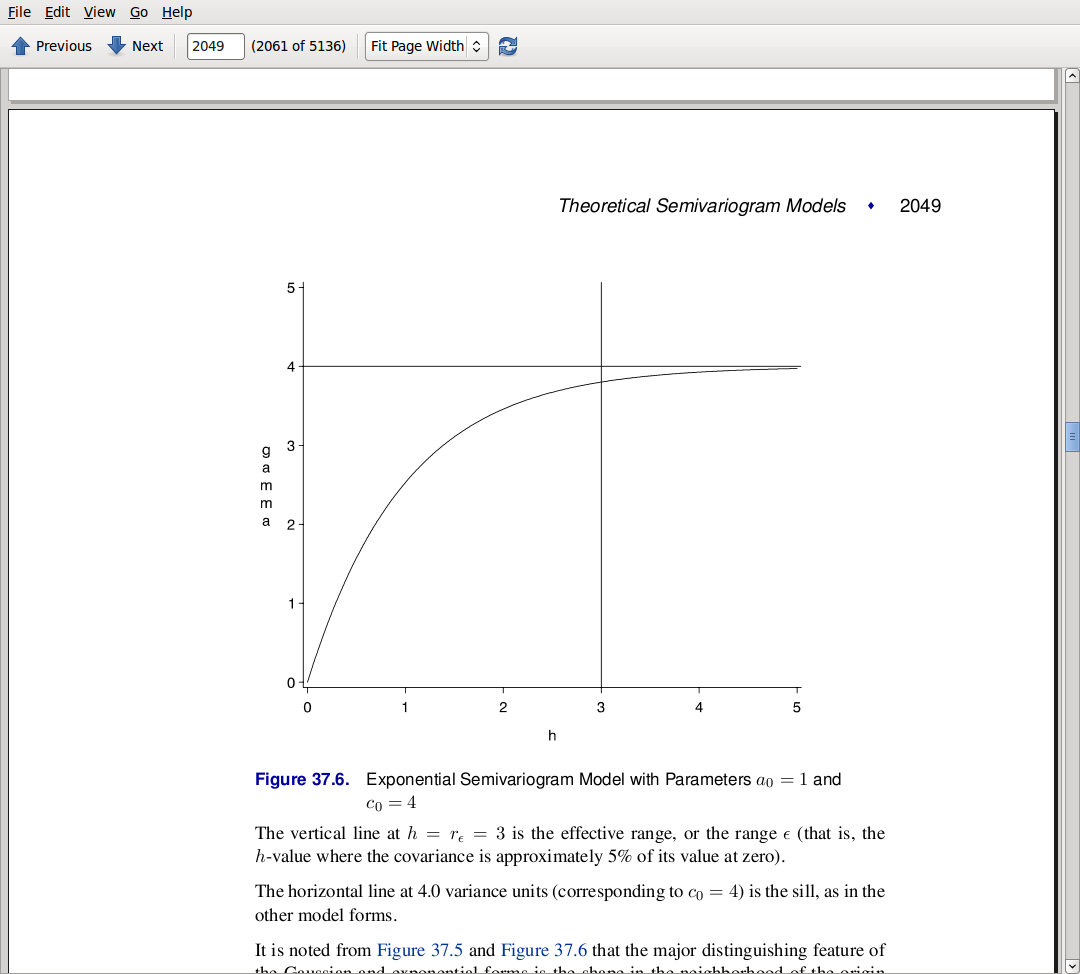
\includegraphics[width=3in]{exponential-model}

Range is 1, scale is 4. (Get range as distance where height is 95\% of
max, divided by 3.)

Rises fast, then approaches limit gradually.

\end{frame}

\begin{frame}{Gaussian}

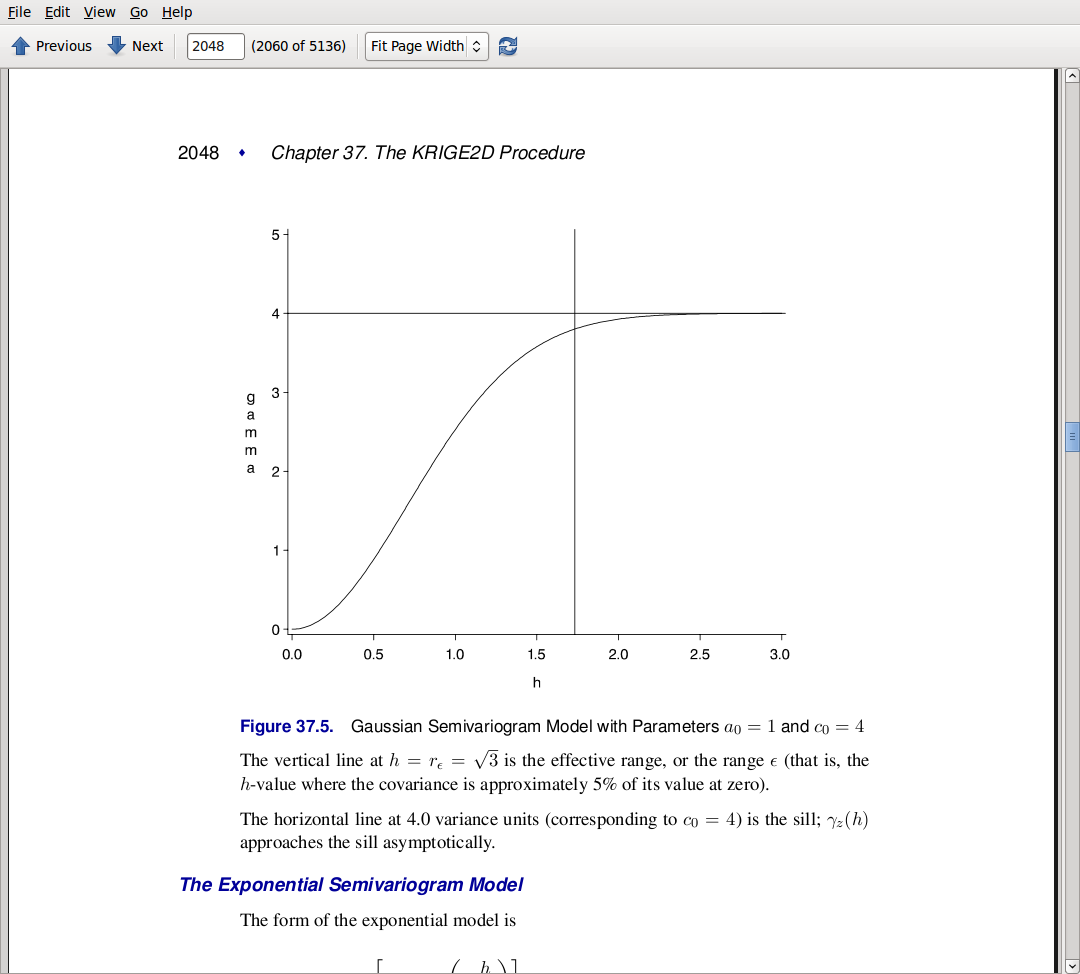
\includegraphics[width=3in]{gaussian-model}

Range is 1, scale is 4. (Range is distance where height is 95\% of
max, divided by 1.7).

Rises slow then faster, approaches limit gradually.

\end{frame}

\begin{frame}[fragile]{Returning to our data}


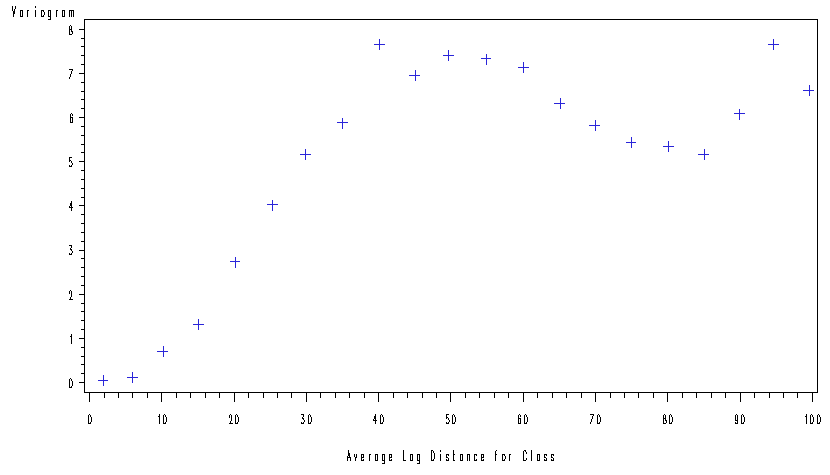
\includegraphics[width=4in]{variog1}

Slow rise at start suggests Gaussian model,  max height (scale) about
7, range about $50/1.7=30$. Feed these into kriging routine.

\end{frame}

\begin{frame}[fragile]{Kriging code}

\begin{verbatim}
proc krige2d data=thick outest=est; 
  coord xc=east yc=north; 
  grid x=0 to 100 by 5 y=0 to 100 by 5; 
  pred var=thick r=10; 
  model scale=7 range=30 form=gauss; 

proc print data = est (obs = 10);

\end{verbatim}
  
\end{frame}

\begin{frame}[fragile]{Output and output data set (part)}

{\scriptsize
\begin{verbatim}
                     Covariance Model Information

                     Type                Gaussian
                     Sill                       7
                     Range                     30
                     Effective Range    51.961524

   Obs     LABEL      VARNAME  GXC  GYC  NPOINTS  ESTIMATE   STDERR

     1  Pred1.Model1   thick    0     0     20     44.0107  0.66714
     2  Pred1.Model1   thick    0     5     20     43.3504  0.65143
     3  Pred1.Model1   thick    0    10     20     42.3169  0.59026
     4  Pred1.Model1   thick    0    15     20     40.9308  0.52172
     5  Pred1.Model1   thick    0    20     20     39.4097  0.36240
     6  Pred1.Model1   thick    0    25     20     37.8804  0.22627
     7  Pred1.Model1   thick    0    30     20     36.3949  0.15932
     8  Pred1.Model1   thick    0    35     20     35.2236  0.10873
     9  Pred1.Model1   thick    0    40     20     33.9929  0.06815
    10  Pred1.Model1   thick    0    45     20     33.2266  0.05748
\end{verbatim}
  }

\end{frame}

\begin{frame}[fragile]{Making plots}

Plot as 3D plot and contour plot:

\begin{verbatim}
    
proc g3d data=est;
  plot gyc*gxc=estimate;
  label gyc      = 'North' 
        gxc      = 'East' 
        estimate = 'Estimated Thickness'; 

proc gcontour data=est;
  plot gyc*gxc=estimate / nlevels=10 autolabel;
  label gyc      = 'North' 
        gxc      = 'East' 
        estimate = 'Estimated Thickness'; 


\end{verbatim}


  
\end{frame}

\begin{frame}{3D plot}
  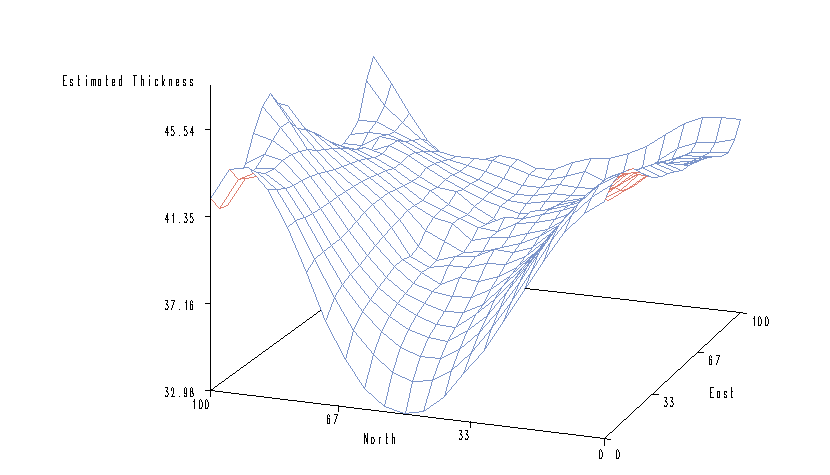
\includegraphics[width=4in]{krige3d}
\end{frame}

\begin{frame}{Contour plot}
  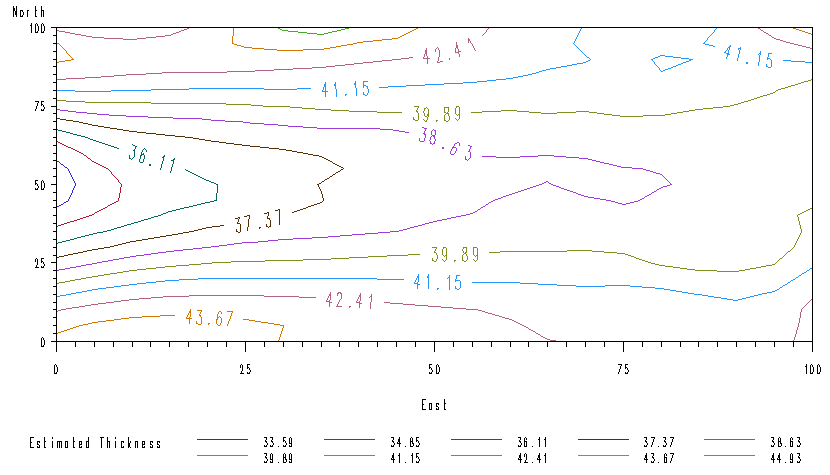
\includegraphics[width=4in]{krigecontour}
\end{frame}

\begin{frame}{Contour plot of SE of estimate}
  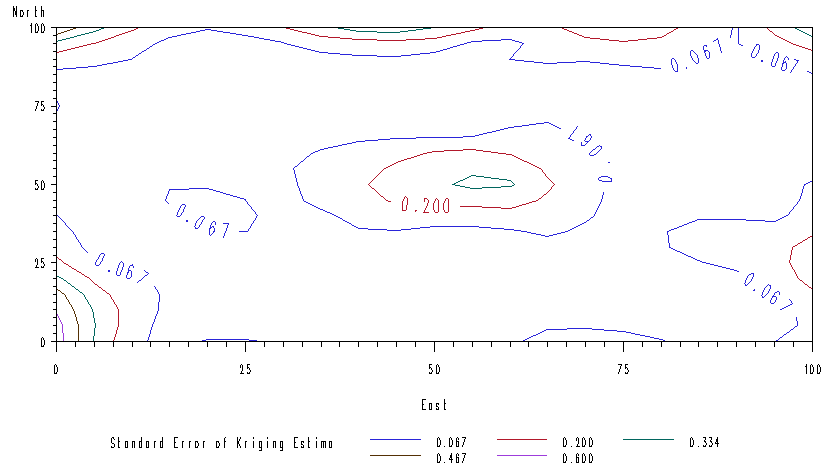
\includegraphics[width=4in]{krigesecontour}
\end{frame}




%%% Local Variables: 
%%% mode: latex
%%% TeX-master: "slides.beamer"
%%% End: 
